\section{Dataflyt fra bilen til brukergrensesnitt}
Hele løsningen rundt å få data fra bilens telemetrimodul til brukeren er realisert med 3 modulerer som gjør hver sin jobb for å frakte dataene.
\begin{figure}[H]
\caption{Dataflyt} 
\label{dataflow}
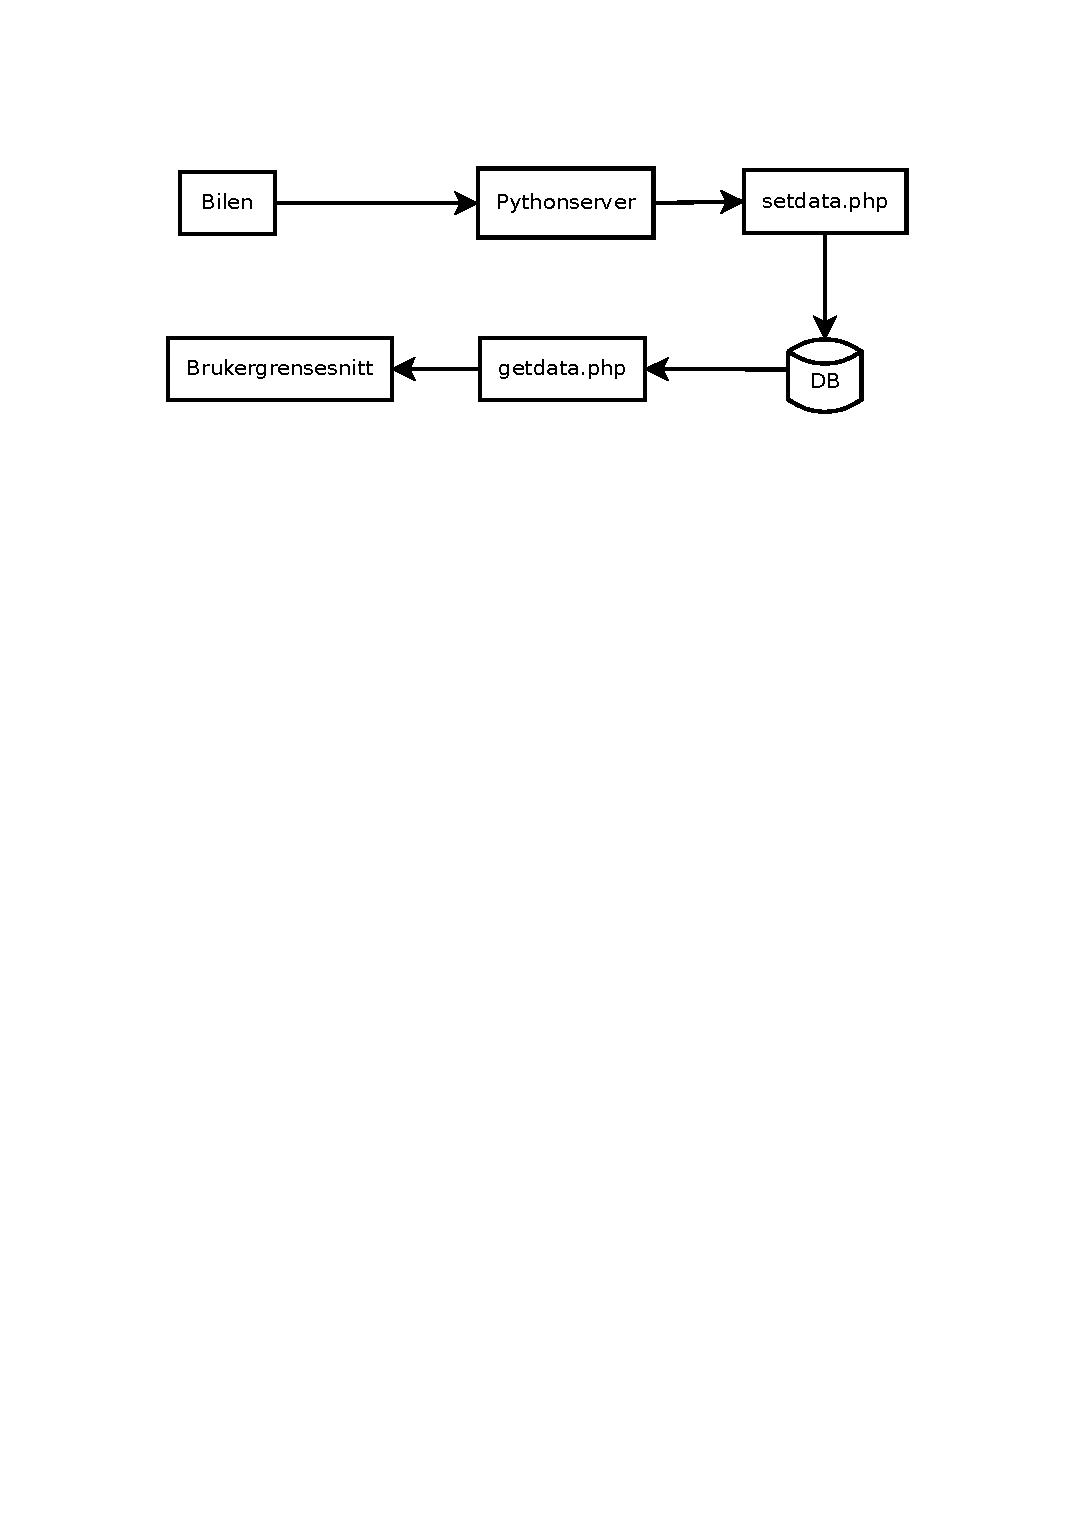
\includegraphics[width=\textwidth, trim=0 550 0 75]{images/dataflow.pdf}
\end{figure}
\subsection{Pythonserver}
Pythonserver er et lite script skrevet i Python som setter opp en TCP socket for å motta data som telemetrimodulen sender. Så fort den har mottatt en hel pakke med data fra bilens telemetrimodul gjør den en omregning av gpsposisjonene fra grader og minutter til rene grader på decimalformat. Deretter sender den dette videre ved å sette opp en HTTP connection til webserveren og sender dataene som et POST request til setdata.php.
\subsection{setdata.php}
Denne modulen tar i mot kommaseparerte data fra Pythonserveren og setter disse inn i databasen. I tillegg gjør den utregninger i forhold til om bilen har passert kontrollpunkt og oppdaterer tidstabellen i henhold til dette.
\subsection{getdata.php}
Denne brukes for å hente data fra databasen når websiden vises. Den slår opp i databasen og bygger opp jquery som igjen oppdaterer elementer i guiet.
\section{Brukergrensesnitt}
Brukergrensesnittet er bygget ut hjelp av noe spesielt rammeverk, men i stedet bygget fra grunnen ved hjelp av PHP, javascript og jquery. Det kjører en jqueryfunksjon som hver x. minutt som henter verdiene som getdata.php genererer og oppdaterer elementene i brukergrensesnittet med det. Brukergrensesnittet har også et kart som bruker api fra google for å sette logoen til fuelfighter på kartet og få den til å bevege seg utifra data fra bilen. En oversikt over hvordan det ferdige systemet ser ut kan sees in en skjermdumpen \ref{gui}.
\begin{figure}[H]
\caption{Ferdig system} 
\label{gui}
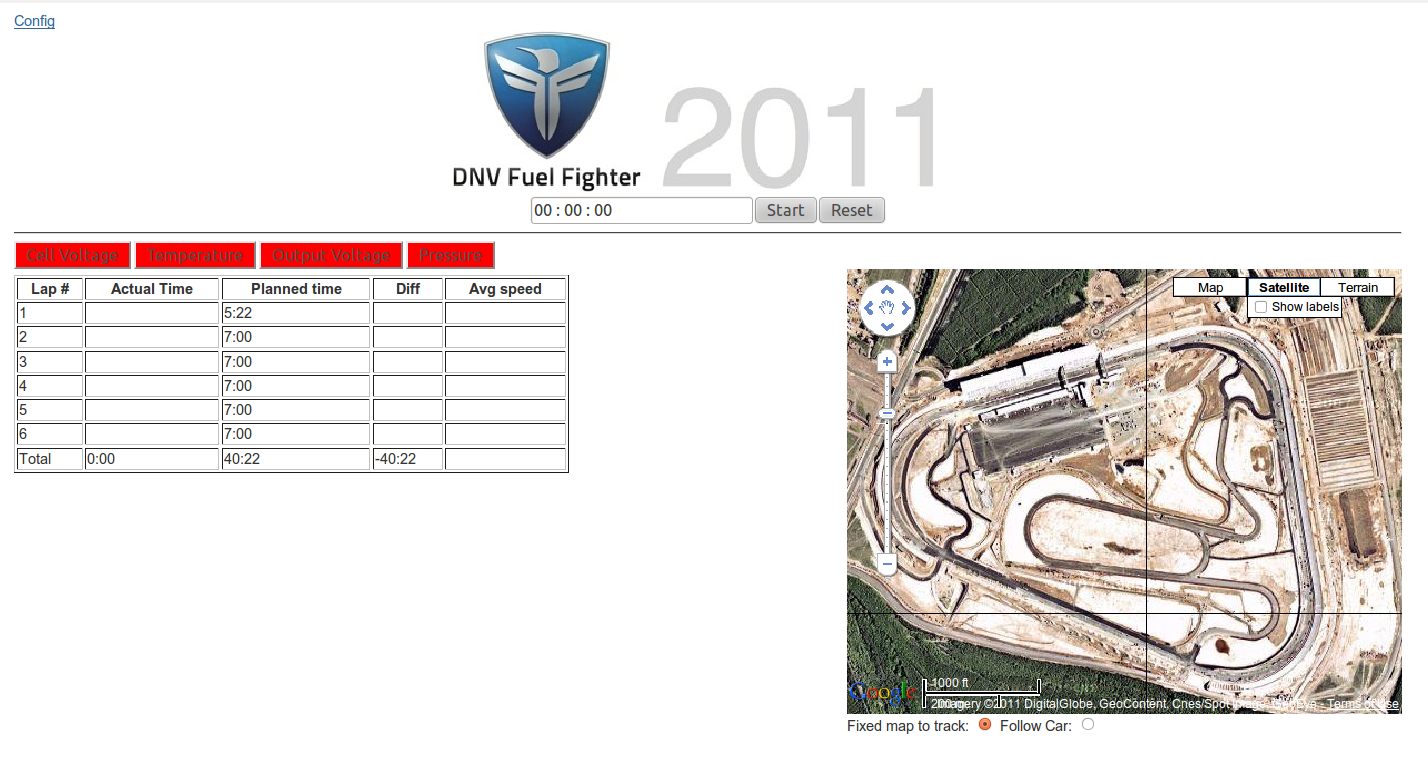
\includegraphics[width=\textwidth]{images/gui.png}
\end{figure}
\subsubsection{Konfigurasjon}
Det finnes også et brukergrensesnitt for at brukeren av systemet skal kunne sette navn, måleenhet og grenseverdi på sensorer. I tillegg kan også planlagte tider og hvor dataene skal hentes fra settes her.
En skjermdump av dette finnes i \ref{config}, dette kommer opp som et vindu over grensesnittet i \ref{gui}.
\begin{figure}[H]
\caption{Config} 
\label{config}
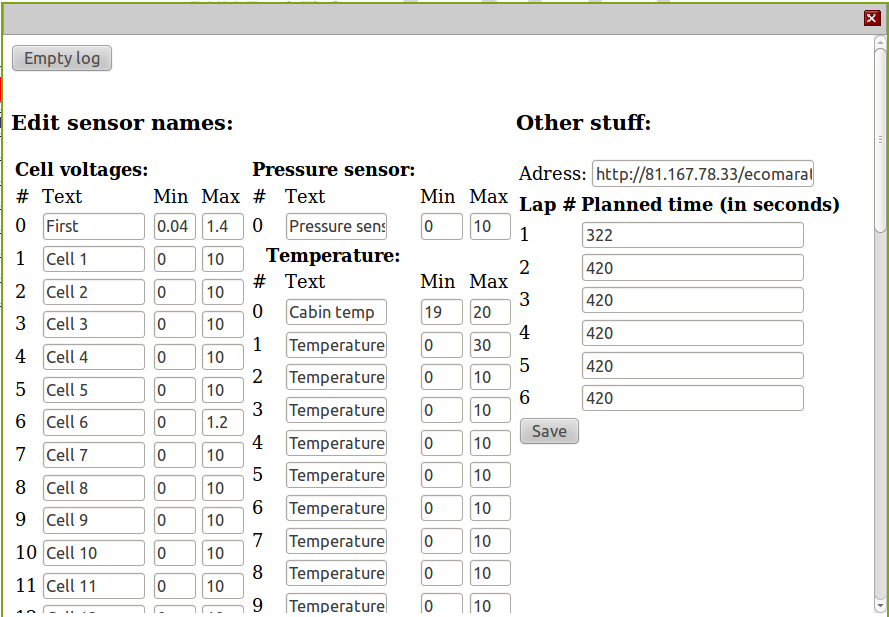
\includegraphics[width=200px]{images/config.png}
\end{figure}

\subsubsection{Statistikk}
Hver sensor kan trykkes på og da kommer vinduet som er vist i \ref{stats} opp, dette genereres ut i fra det som blir lagt inn av setdata.php. Her kan man navigere frem og tilbake i historien for å finne ut når en sensor har meldt om feil.
\begin{figure}[H]
\caption{Statistikk} 
\label{stats}
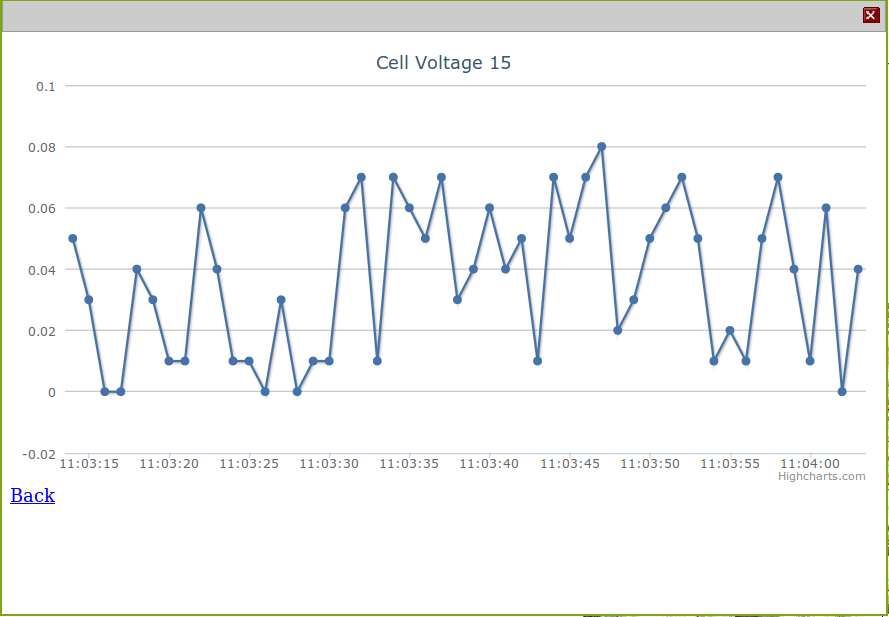
\includegraphics[width=200px]{images/stat.png}
\end{figure}
\section{Telemetrimodul}
Telemtrimodulen ble laget av Anders Guldahl \cite{telemetrithesis} i 2009. Denne har ikke blitt endret mye på, men noen endringer måtte gjøres for at den skulle fungere sammen med brukergrensesnittet.
Slik det var, så leverte telemetrimodulen GPS data kun til dashbordet i bilen og hastigheten til bilen ble aldri brukt. Dette er nå endret slik at telemetrimodulen sender disse dataene sammen med de andre måleverdiene som en komma separert string via GPRS til Pythonserveren.
